% $Id: template.tex 11 2007-04-03 22:25:53Z jpeltier $

%\documentclass{vgtc}                          % final (conference style)
%%\documentclass[review]{vgtc}                 % review
%%\documentclass[widereview]{vgtc}             % wide-spaced review
%%\documentclass[preprint]{vgtc}               % preprint
%%\documentclass[electronic]{vgtc}             % electronic version
%
%% Added by KM, 130928, to get it to compile. Not sure why.
%\let\ifpdf\relax
%
%
%%% Uncomment one of the lines above depending on where your paper is
%%% in the conference process. ``review'' and ``widereview'' are for review
%%% submission, ``preprint'' is for pre-publication, and the final version
%%% doesn't use a specific qualifier. Further, ``electronic'' includes
%%% hyperreferences for more convenient online viewing.
%
%%% Please use one of the ``review'' options in combination with the
%%% assigned online id (see below) ONLY if your paper uses a double blind
%%% review process. Some conferences, like IEEE Vis and InfoVis, have NOT
%%% in the past.
%
%%% Figures should be in CMYK or Grey scale format, otherwise, colour 
%%% shifting may occur during the printing process.
%
%%% These three lines bring in essential packages: ``mathptmx'' for Type 1 
%%% typefaces, ``graphicx'' for inclusion of EPS figures. and ``times''
%%% for proper handling of the times font family.
%
%\usepackage{mathptmx}
%\usepackage{graphicx}
%\usepackage{times}
%
%% K additions (commenting)
%\usepackage{xcolor}
%%\usepackage{pdfcomment}
%
%%% We encourage the use of mathptmx for consistent usage of times font
%%% throughout the proceedings. However, if you encounter conflicts
%%% with other math-related packages, you may want to disable it.
%
%%% If you are submitting a paper to a conference for review with a double
%%% blind reviewing process, please replace the value ``0'' below with your
%%% OnlineID. Otherwise, you may safely leave it at ``0''.
%\onlineid{0}
%
%%% declare the category of your paper, only shown in review mode
%\vgtccategory{Research}
%
%%% allow for this line if you want the electronic option to work properly
%\vgtcinsertpkg
%
%
%% sort citations
%\usepackage{cite}
%%\usepackage[sort]{natbib}
%
%
%%% =================================
%% inline comments[KM addition]
%\definecolor{DarkGreen}{rgb}{0.0, 0.6, 0.0}
%\definecolor{DarkRed}{rgb}{0.7, 0.2, 0.2}
%\definecolor{DarkMagenta}{rgb}{0.5, 0.0, 0.5}
%\definecolor{DarkCyan}{rgb}{0.0, 0.6, 0.6}
%
%%\newcommand{\inlinecomment}[3][]{$\lceil$\textbf{#1}~\textit{\textcolor{#2}{#3}}$\rfloor$}
%\newcommand{\inlinecomment}[3][]{\textbf{#1}~\textit{\textcolor{#2}{#3}}}
%
%\newcommand{\todo}[1]{\noindent \inlinecomment[TODO]{DarkRed}{#1}}
%\newcommand{\km}[1]{\noindent \inlinecomment{DarkGreen}{#1}}
%\newcommand{\ikComment}[1]{\noindent \inlinecomment[IK]{DarkCyan}{#1}}
%\newcommand{\bgComment}[1]{\noindent \inlinecomment[BG]{blue}{#1}}
%
%
%\newcommand{\kmEdit}[1]{\textcolor{DarkGreen}{#1}}
%% \newcommand{\grn}[1]{\textcolor{DarkGreen}{#1}}
%%% =================================
%
%

\chapter{Improvise: The Haptic Instrument}
\label{ch:hapticinstrument}


%% In preprint mode you may define your own headline.
%\preprinttext{To appear in an IEEE VGTC sponsored conference.}

%% Paper title.

%\title{Haptic Jazz: Designing Touch with the Haptic Instrument}
%\title{Improvising Design with a Haptic Instrument}

%% This is how authors are specified in the conference style

%% Author and Affiliation (single author).
%%\author{Roy G. Biv\thanks{e-mail: roy.g.biv@aol.com}}
%%\affiliation{\scriptsize Allied Widgets Research}

%% Author and Affiliation (multiple authors with single affiliations).
%%\author{Roy G. Biv\thanks{e-mail: roy.g.biv@aol.com} %
%%\and Ed Grimley\thanks{e-mail:ed.grimley@aol.com} %
%%\and Martha Stewart\thanks{e-mail:martha.stewart@marthastewart.com}}
%%\affiliation{\scriptsize Martha Stewart Enterprises \\ Microsoft Research}

%% Author and Affiliation (multiple authors with multiple affiliations)
\author{Oliver S. Schneider\thanks{e-mail: oschneid@cs.ubc.ca} \qquad \qquad Karon E. MacLean\thanks{e-mail: maclean@cs.ubc.ca}\\ %
        \scriptsize Department of Computer Science \\
        \scriptsize University of British Columbia, Vancouver, Canada
}
%\author{Oliver S. Schneider\thanks{e-mail: oschneid@cs.ubc.ca}\\ %
%        \scriptsize University of British Columbia %
%\and Karon E. MacLean \thanks{e-mail: maclean@cs.ubc.ca}\\ %
%        \scriptsize University of British Columbia %
%%\and Martha Stewart\thanks{e-mail:martha.stewart@marthastewart.com}\\ %
%%     \parbox{1.4in}{\scriptsize \centering Martha Stewart Enterprises \\ Microsoft Research}
%}

%% A teaser figure can be included as follows, but is not recommended since
%% the space is now taken up by a full width abstract.
%\teaser{
%  \includegraphics[width=1.5in]{sample.eps}
%  \caption{Lookit! Lookit!}
%}

%%\abstract{
%% Designing haptic phenomena is increasingly important but difficult.
%As the need to deploy informative, expressive haptic phenomena in consumer devices gains momentum, the inadequacy of current design tools is becoming more critically obstructive.
%%However, this increased activity  also makes it possible to characterize issues, and address them with advances in software engineering.
%%Designers face two primary obstacles.
%Current tools do not support collaboration or serendipitous exploration.
%Collaboration is critical,
%but direct means of sharing haptic sensations are limited,
%and the absence of unifying conceptual models for working with haptic sensations further restricts communication between designers and stakeholders.
%%Because there are no unifying conceptual models for working with haptic sensations, there are major communication problems between designers and stakeholders.
%%: neither designers, nor managers, nor users can articulate what they experience.
%%This is especially troublesome when designing pleasant, affective interactions that rely upon user experience.
%This is especially troublesome for pleasurable, affectively targeted interactions that rely on 
%subjective user experience.
%%In this paper, we introduce our solution: the haptic instrument, analogous to a musical instrument, a new tool for real-time, collaborative manipulation of haptic sensations.
%In this paper, we introduce an alternative design approach
%inspired by musical instruments -- a new tool for real-time, collaborative manipulation of haptic sensations;
%and describe % the design of 
%a first example, mHIVE, a mobile Haptic Instrument for Vibrotactile Exploration.
%%, which allows both designers and users to express vibrotactile \km{(VT)} ideas with a simple touchscreen interface.
%Our qualitative study shows that mHIVE supports exploration and communication but
%requires additional visualization and recording capabilities for tweaking designs,
%and expands previous work on haptic language.
%%and reveals future research directions for both design tools and language.
%%}


%% ACM Computing Classification System (CCS). 
%% See <http://www.acm.org/class/1998/> for details.
%% The ``\CCScat'' command takes four arguments.
%
%\CCScatlist{
%  \CCScat{H.5.2}{Information Interfaces and Presentation (e.g., HCI)}{User Interfaces}{Haptic I/O}
%}

%% Copyright space is enabled by default as required by guidelines.
%% It is disabled by the 'review' option or via the following command:
% \nocopyrightspace

%%%%%%%%%%%%%%%%%%%%%%%%%%%%%%%%%%%%%%%%%%%%%%%%%%%%%%%%%%%%%%%%
%%%%%%%%%%%%%%%%%%%%%% START OF THE PAPER %%%%%%%%%%%%%%%%%%%%%%
%%%%%%%%%%%%%%%%%%%%%%%%%%%%%%%%%%%%%%%%%%%%%%%%%%%%%%%%%%%%%%%%%

% Make sure hyperref comes last of your loaded packages, 
% to give it a fighting chance of not being over-written, 
% since its job is to redefine many LaTeX commands.
%\usepackage[pdftex]{hyperref}
%\hypersetup{
%pdftitle={SIGCHI Conference Proceedings Format},
%pdfauthor={LaTeX},
%pdfkeywords={SIGCHI, proceedings, archival format},
%bookmarksnumbered,
%pdfstartview={FitH},
%colorlinks,
%citecolor=black,
%filecolor=black,
%linkcolor=black,
%urlcolor=black,
%breaklinks=true,
%}


%Set graphics path

%% create a shortcut to typeset table headings
%\newcommand\tabhead[1]{\small\textbf{#1}}
%
%%new command that is a bold item
\newcommand\strongitem[1]{{\textbf{#1.}}}
%
%%new command that describes a theme:
\newcounter{themecounter}
\stepcounter{themecounter}
%%\newcommand\theme[1]{\vspace{2mm}\textbf{Theme \thethemecounter: #1}\stepcounter{themecounter}}
%%\newcommand\theme[1]{\subsection{Theme \thethemecounter: #1}\stepcounter{themecounter}}
\newcommand\theme[1]{\subsection{#1}}

%quote commands
\newcommand\q[1]{\textit{``#1"}} 			%\q for quote
\newcommand\sq[1]{{\q{#1}}}			%\sq for small quote
\newcommand\namedquote[2]{{\q{#2} (#1)}}
%\newcommand\namedquote[2]{{\textbf{#1:} \q{#2}}}
\newcommand\nq[2]{\namedquote{P#1}{#2}}	%\nq for named quote of participant number N
\newcommand\term[1]{\textit{#1}} 			%\term

%\numberofauthors{1}
%%\author{
%%  \alignauthor Author(s) Name(s)\\
%%    \affaddr{Affiliation(s)}\\
%%    \affaddr{Address(es)}\\
%%    \email{e-mail address(es)}\\
%%    \affaddr{Optional phone number(s)}
%%}
%
%
%%\keywords{
%%	vibrotactile; design tools;
%%	\textcolor{red}{Mandatory section to be included in your final version.}
%%}
%
%%\category{H.5.m.}{Information Interfaces and Presentation (e.g. HCI)}{Miscellaneous}
%%See: \url{http://www.acm.org/about/class/1998/}
%%for more information and the full list of ACM classifiers
%%and descriptors.
%
%\begin{document}
%% The ``\maketitle'' command must be the first command after the
%% ``\begin{document}'' command. It prepares and prints the title block.

%% the only exception to this rule is the \firstsection command

%%%%%%%%%%%%%%%%%%
%
% SECTION: Introduction
% 
%%%%%%%%%%%%%%%%%%
%\section{Introduction}

%%\maketitle
%
%Haptic feedback has hit %devices  are hitting 
%the mainstream, present in smartphones, gaming and automobile design,
%%Everything from smartphones to cars are adopting higher-fidelity haptic technology.
%but our knowledge of how to design haptic phenomena remains limited.
%%Despite years of research
%There are still no agreed-upon vocabularies or conceptual models for haptic phenomena \cite{Enriquez2003,Ledo2012,Lee2009,Obrist2013}, % putting \km{us} % haptic design at a loss when compared 
%in contrast to other modalities (\emph{e.g.}, using theory of minor chords to evoke a sad emotion in music).
%% Prospects are even more limited when developing sensations to have qualitative features, such as pleasant alerts or frightening game environments.
%For subjective qualities, such as pleasant alerts or frightening game environments, prospects are even more limited.
%%
%Design is still based on trial and error with programming languages, limiting exploration.
%%Programming languages are primarily used, limiting exploration.
%The lack of established conceptual models or design frameworks further challenges communication between designers and stakeholders.
%%The subset of tactile sensations has a number of candidates (e.g., vibrotactile score \cite{Lee2009}), but even this area can be improved.
%%In particular, existing tools fail to support designers in two ways:
%
%%\begin{itemize}
%%	\item Development cycles are still based on compile, run, adjust cycles, or hardware vendor demos/examples
%%	\item There is no understood mental model or design theory when creating haptic phenomena
%%\end{itemize}
%

%\begin{figure}[th] %  figure placement: here, top, bottom, or page
%   \centering
%   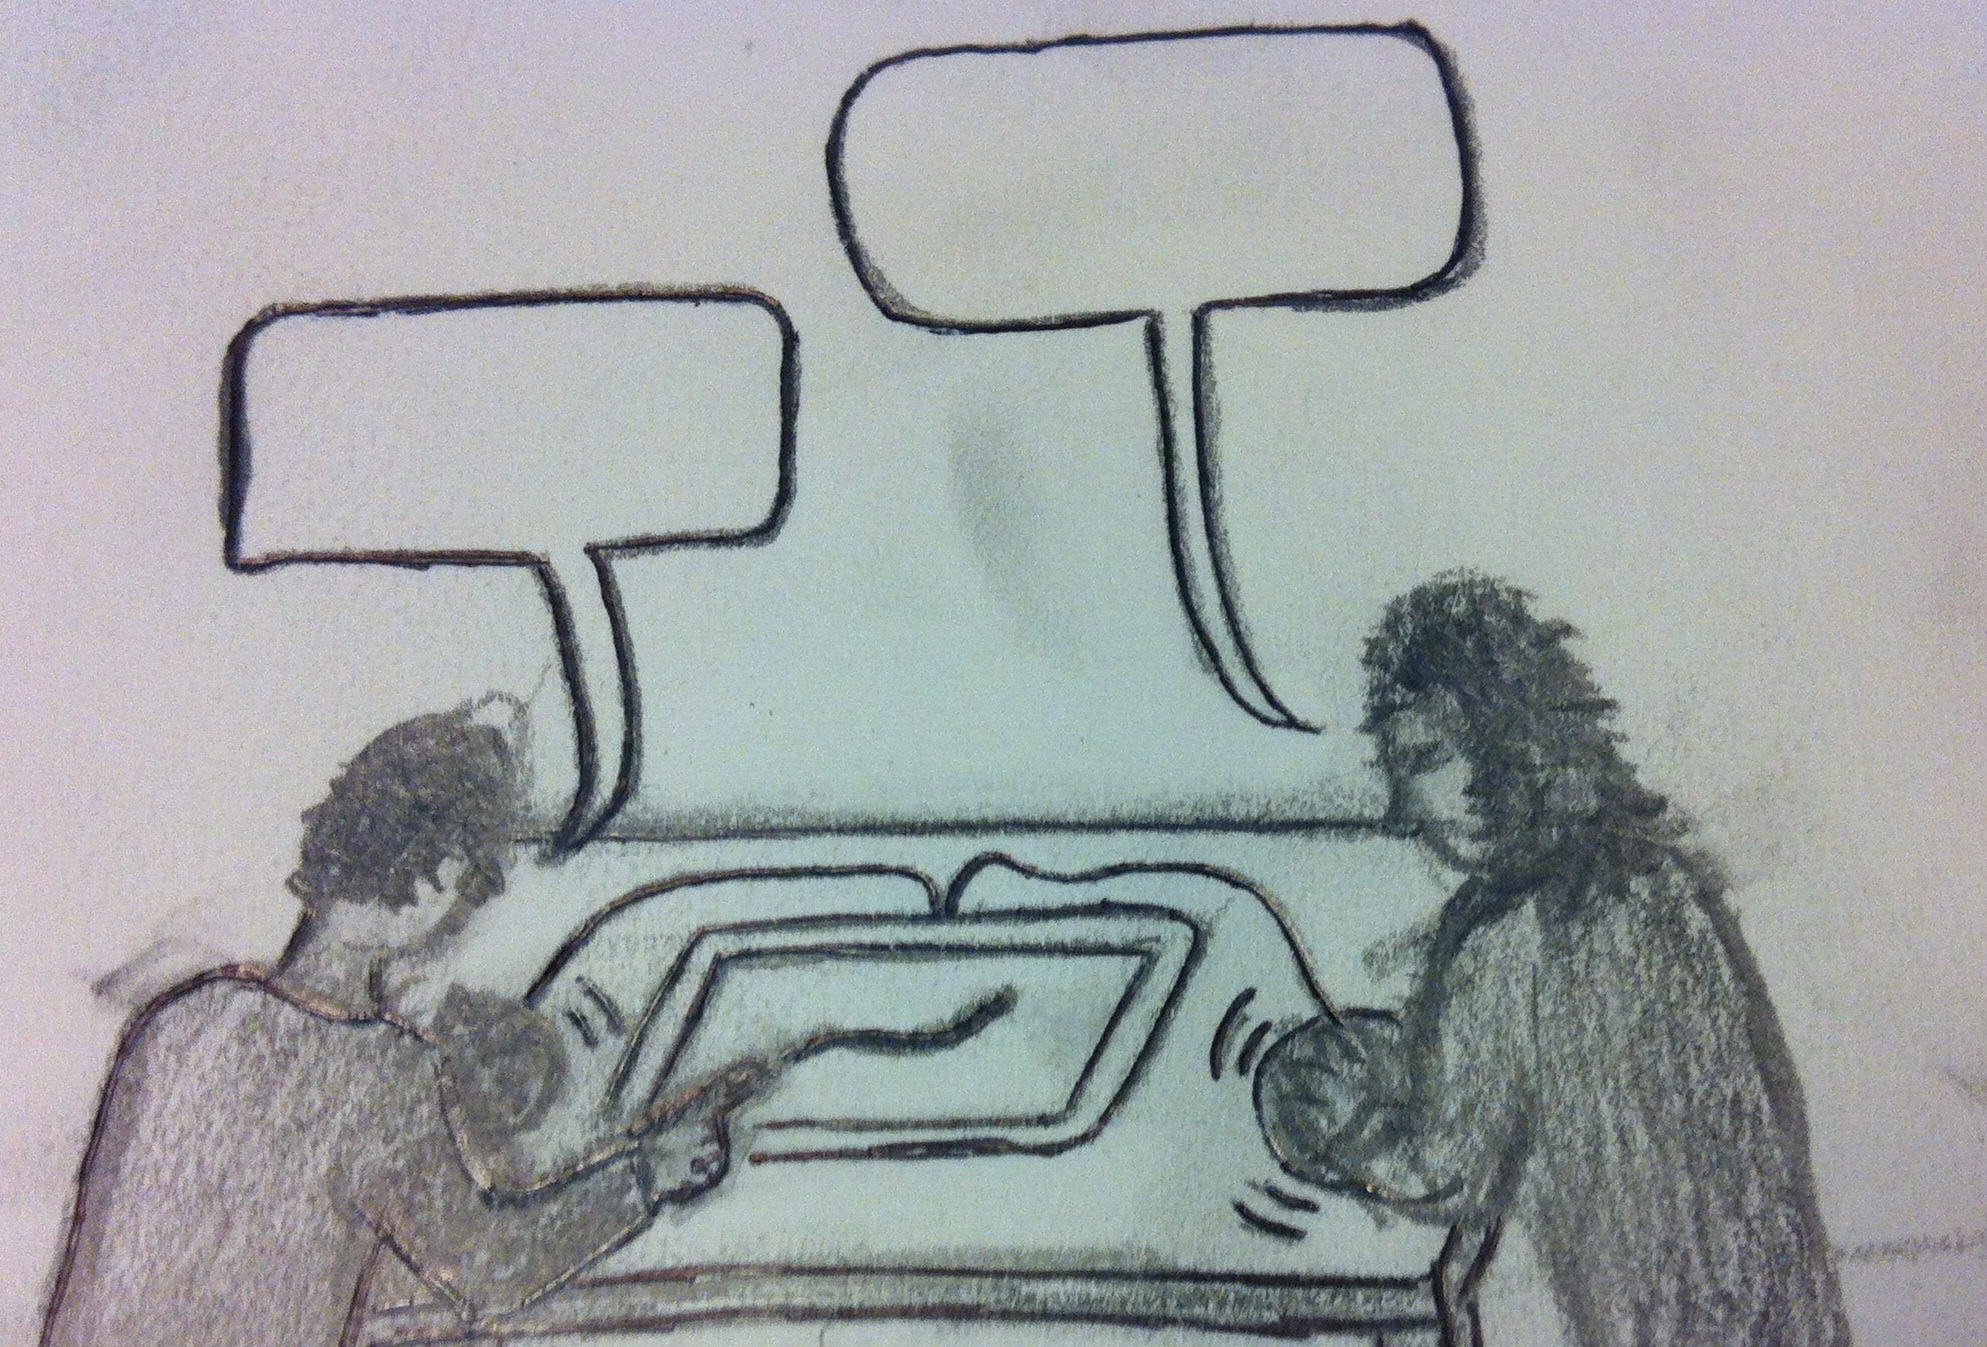
\includegraphics[width=0.4\textwidth]{HapticInstrumentConceptSketchRough} 
%   \caption{Concept Sketch of the Haptic Instrument}
%   \label{fig:HapticInstrumentConceptSketch}
%\end{figure}

\begin{figure}[h] %  figure placement: here, top, bottom, or page
   \centering
   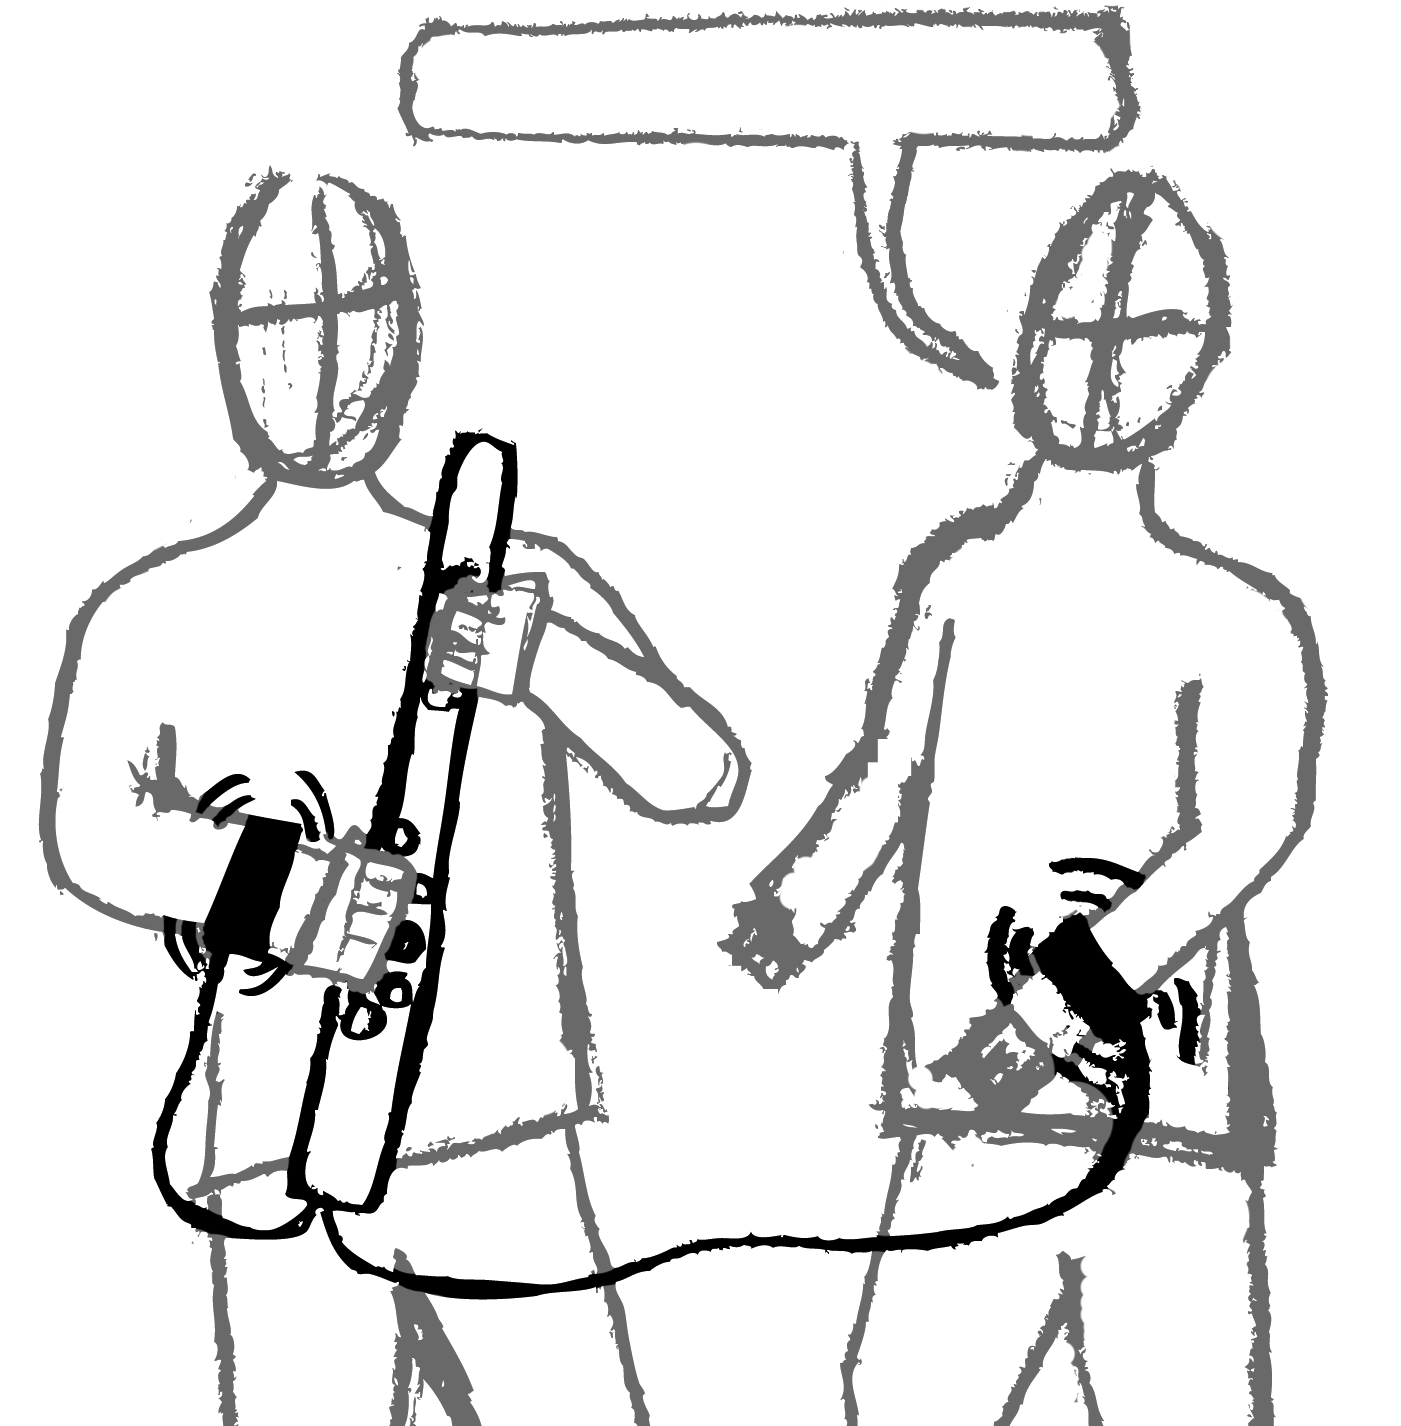
\includegraphics[width=0.5\textwidth, height=2.3in]{haptic-instrument-concept-sketch-sax-small-traced-squarer} 
   \caption{Concept sketch of a haptic instrument. Both users are experiencing the same sensation, controlled in real-time.}
   \label{fig:HapticInstrumentConceptSketch}
\end{figure}

The Haptic Instrument case study\footnote{Published in Haptics Symposium 2014 \cite{Schneider2014} and at a CHI 2014 workshop \cite{Schneider2014b}.} investigates the role of real-time feedback and synchronous collaboration on haptic experience design, using participants with some haptics experience, serving as proxies for haptic experience designers.
Conventional haptic design tools contain a slow iteration, requiring programming or rendering before playback.
Using a music composition metaphor (as in~\cite{Lee2009}), we are writing music without ever playing a note: composing a work in its entirety, then listening to the result before making changes.
In contrast, musicians often use their instruments as a tool for serendipitous exploration when designing music.
%and can draw upon musical theory.
Furthermore, music is collaborative, with communication facilitated by a reference point of a sound.
%Touch, however, is a personal, local sense, making it difficult to discuss stimuli.


%Facilitated exploration and collaboration % in haptic design should 
%should streamline the haptic design process and inform a guiding 
%theory, analogous to those for musical composition. % theory. % vague?
%% With eased exploration, 
%Designers will attain fluency with new devices and control parameters,
%while collaborative elements % should help communication, but also 
%% could prove key to developing this theory.
%%Previous approaches have all been single-user design tools.
%%We suspect that adding a collaborative element is the key to developing these languages
%will get people designing in groups.  A usable haptic language may emerge from their dialogue.
%% they use to collaborate might emerge naturally from the collaborative interactions.


%Furthermore, recent work has identified major communication barriers in industry. Designers of haptic sensations are forced to carry examples of different textures or dynamical systems to make their point to stakeholders.



Our approach is to directly use a \emph{haptic instrument}, inspired by musical instruments but producing (for example) vibrotactile (VT) sensations rather than sound (\autoref{fig:HapticInstrumentConceptSketch}).
Haptic instruments are intended to have two main uses: they provide real-time feedback to the user to facilitate improvisation and exploration, and produce haptic output to multiple users as a \emph{what-you-feel-is-what-I-feel} (WYFIWIF) interface.
This allows for a dialogue that includes a haptic modality: haptic instruments create a shared experience of touch, allowing for a common reference point.


% when two or more people are talking.
%We hope that haptic instruments will not only prove to be useful tools in their own right, but also allow for a haptic language to emerge naturally from the dialogue surrounding this shared experience.
%We developed a vibrotactile instance, mHIVE (mobile Haptic Instrument for Vibrotactile Exploration), as a platform to investigate this concept.


%Our main contributions are:
%\begin {itemize}
%	\item A definition of the haptic instrument concept \& design space.
%	\item A fully-working haptic instrument (mHIVE).
%	\item The novel application of an established psychological methodology, phenomenology, to investigate mHIVE's interface and subjective tactile experiences.
%%	rather than psychophysical thresholds.
%	\item Preliminary results from a qualitative study that show mHIVE supports exploration and collaboration, and implications for the design of future haptic design tools.
%\end{itemize}

%%\noindent
%In this paper, we first cover the related work of haptic design tools and haptic language,
%%, identifying the progress so far in haptic design tools and conceptual models.
% then define the haptic instrument, its requirements, features, and design space.
%We report the design of mHIVE,
%% and the feedback we have encountered.
%our methodology, and preliminary results, and
%% investigating both the experience of using mHIVE and the language used to describe haptic phenomena.
% conclude with future directions for haptic tool design and research into a haptic language.
%%, and a vision for how haptic instruments can be used to develop a conceptual framework, the analogous musical theory for haptic sensations.
%%
%%\begin{itemize}
%%	\item Haptic jazz is a rich metaphor
%%	\item Haptic ``lead sheets" instead of scores
%%	\item improvisation
%%	\item social
%%\end{itemize}

%\begin{figure*}[Hb]
%   \centering
%   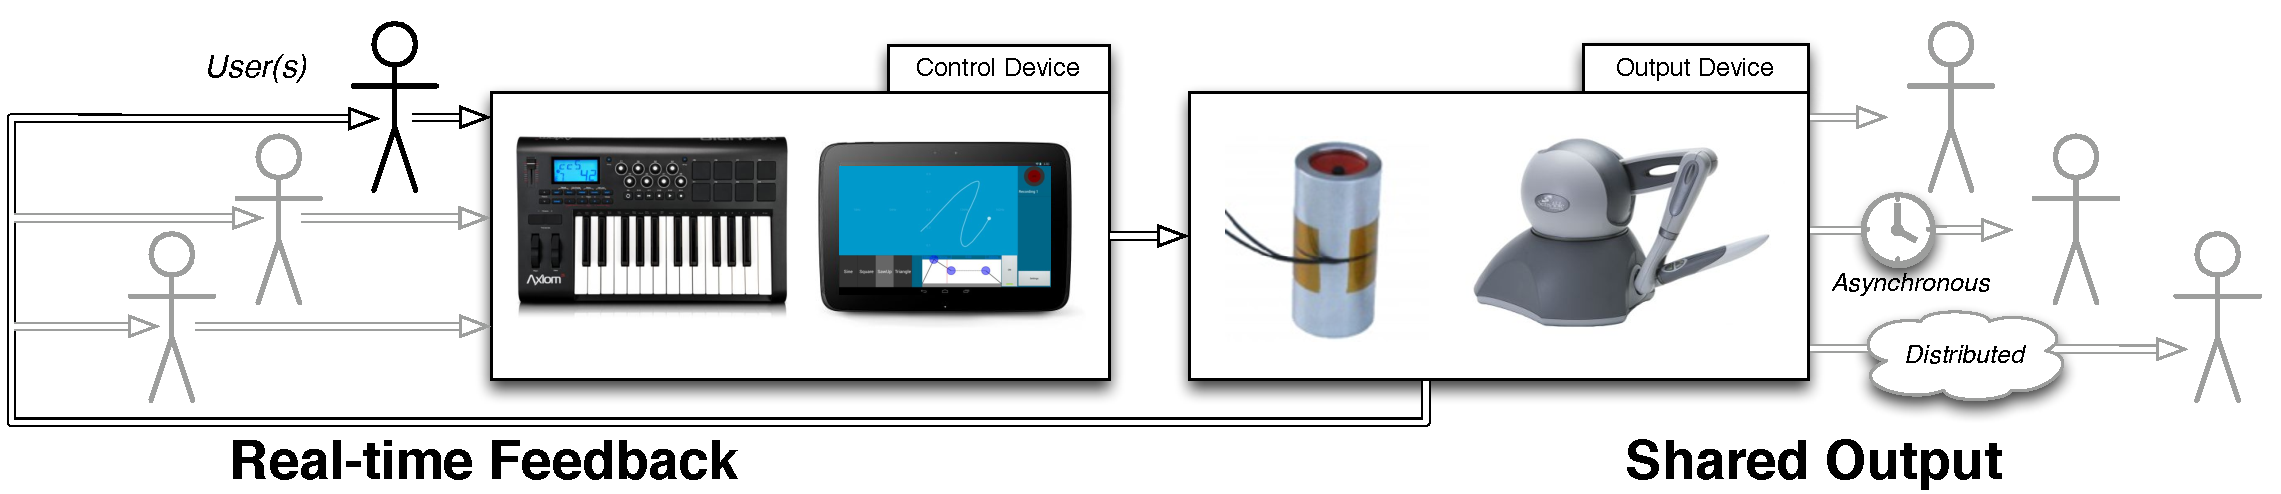
\includegraphics[width=\textwidth]{haptic-instrument-concept-horizontal4-small} 
%   \caption{The haptic instrument concept. One or more people can control the instrument, and receive real-time feedback from the device. Any number of audience members can feel the output in real time as well. Control methods can vary, from traditional musical control devices (such as the M-Audio Axiom 25, used in preliminary prototypes) to touchscreen tablets (used in mHIVE). Output devices vary as well.}
%   \label{fig:HapticInstrumentConcept}
%\end{figure*}




%Finally, we draw inspiration the Logo, which uses the ``transitionary object" of a turtle \cite{Papert1980}??? to aid users in making  to communicate experience, live coding ? Programming by example, haptic camera line of thought?


%%%%%%%%%%%%%%%%%%
%
% SECTION: Defining the Haptic Instrument
% 
%%%%%%%%%%%%%%%%%%
%\section{Defining the Haptic Instrument}
%We define a haptic instrument as a tool for general manipulation of one or more haptic (tactile, force-feedback, or both) devices that provides real-time feedback to anyone controlling the device, and can produce identical shared (WYFIWIF) output to all users to facilitate discussion and collaboration.
%Manipulation can include ideation, exploration, communication, recording, refinement, and articulation.
%Manipulation can be for utilitarian purposes (\emph{e.g.}, designing haptic notifications) or artistic expression (\emph{e.g.}, a haptic performance).
%Output devices can be purely output, or interactive.
%Furthermore, although haptic devices must be involved, multimodal experiences could easily be created by combining a haptic instrument with auditory or visual output.\footnote{One could even imagine a multimodal instrument such as Asimov's Visi-Sonor \cite{Asimov-Foundation-and-Empire} or its parody, Futurama's Holophonor \cite{Futurama-33-ParasitesLost}.}


%\begin{figure*}[htb]
%   \centering
%   \begin{minipage}{0.65\textwidth}
%	   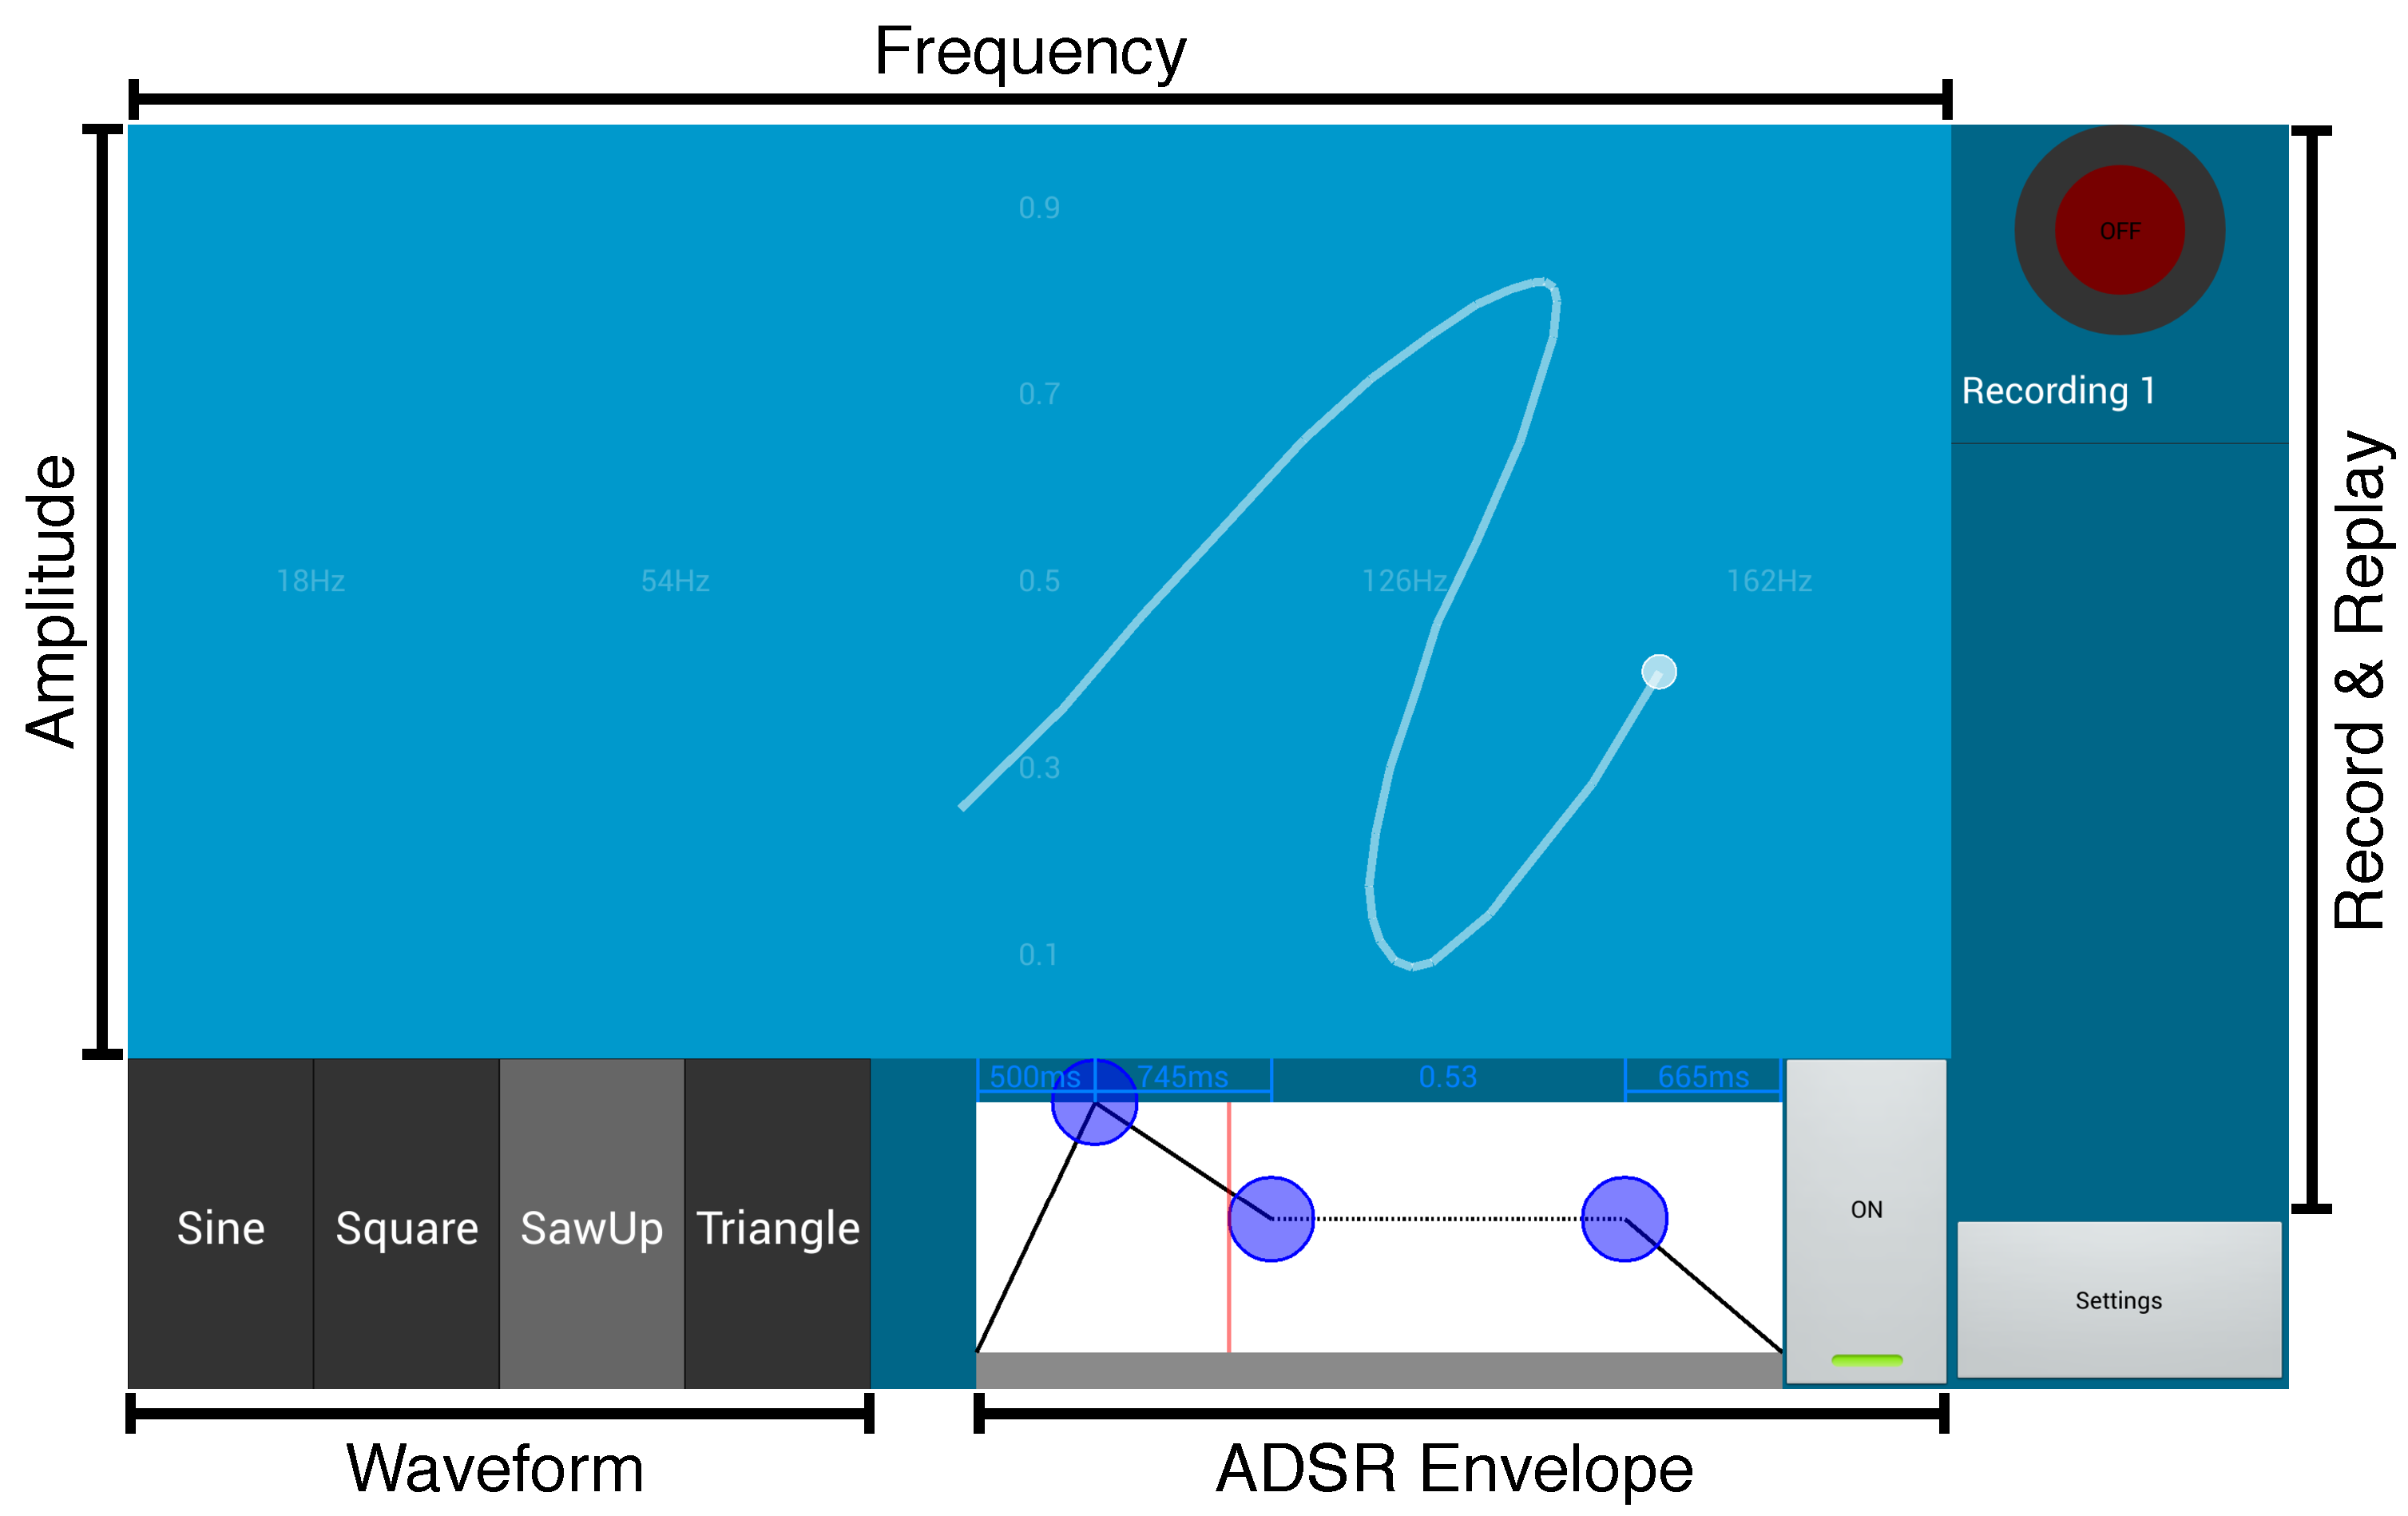
\includegraphics[width=\textwidth]{mHIVE-screenshot-labeled-2013-08-13} 
%	   \caption{mHIVE interface. Primary interaction is through the amplitude-frequency view, where visual feedback is provided through a circle (current finger position) and a trail (two seconds of previous interaction history).}
%	   \label{fig:mHIVE}
%    \end{minipage}
%    \hspace{1cm}
%   \begin{minipage}{0.25\textwidth}
%	   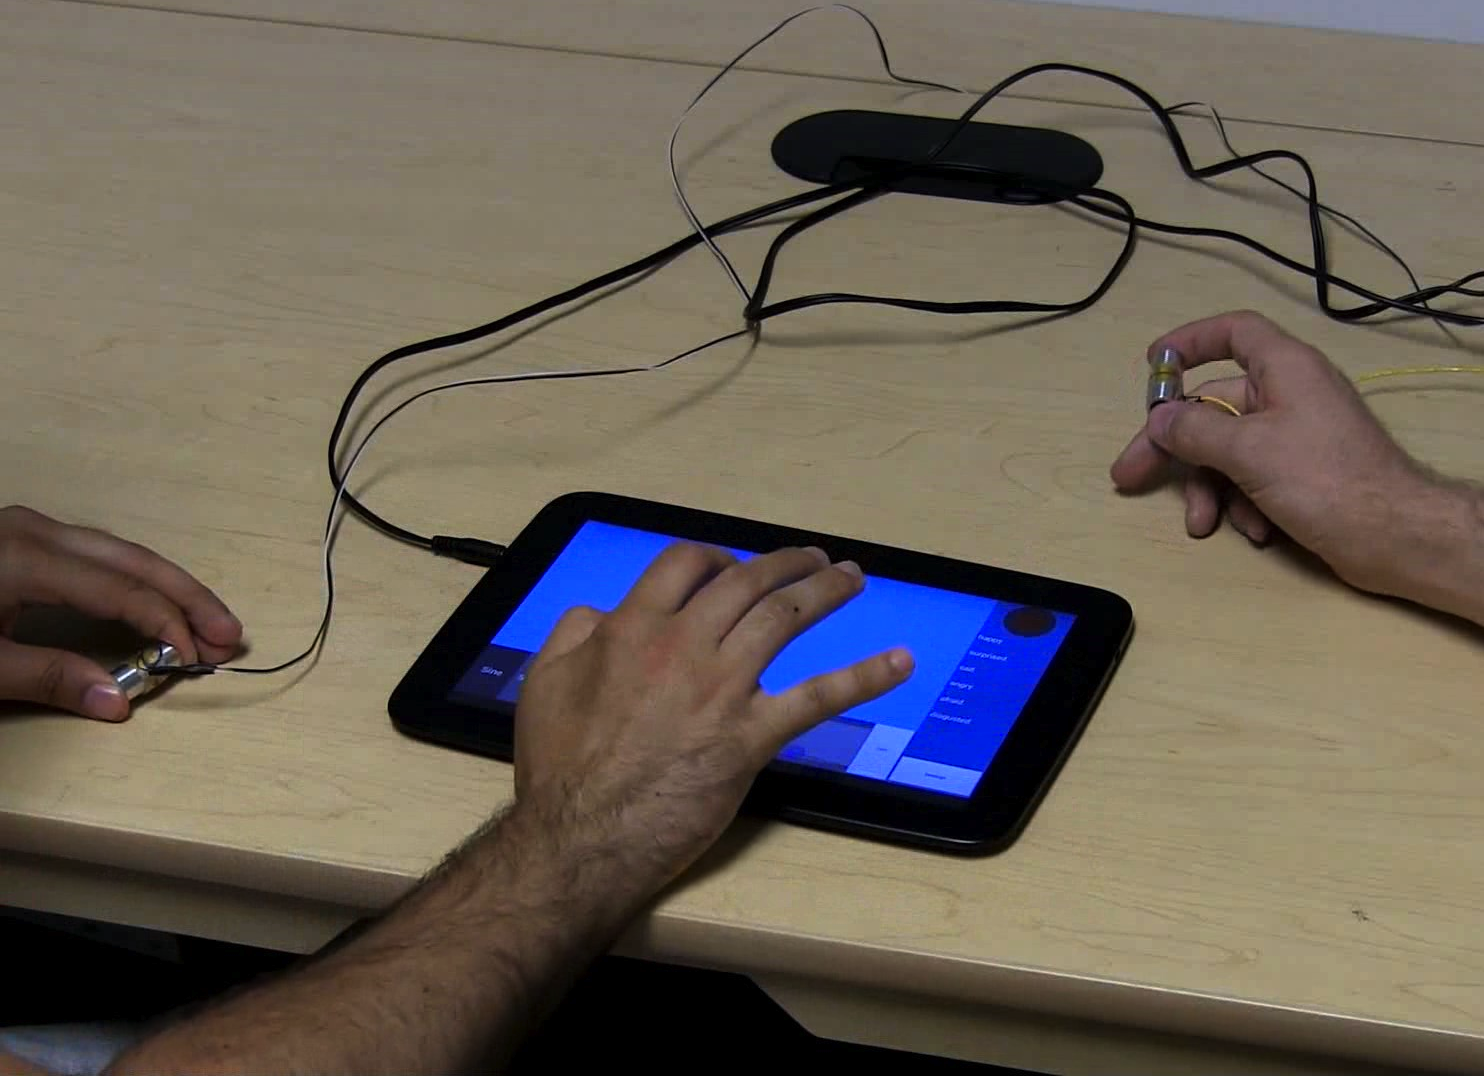
\includegraphics[width=\textwidth]{mHIVE-study-setup-cropped} 
%	   \caption{Study setup. The participant (left) controls the device while feeling the sensation; the interviewer (right) feels the same sensation on an identical output device.}
%	   \label{fig:StudySetup}
%    \end{minipage}   
%\end{figure*}





%%%%%
%SubSection: Design Dimensions
%%%%
%\subsection{Design Dimensions}
%%Though haptic instruments by definition provide real-time feedback have shared-output, there are several main design dimensions that can be considered in a haptic instrument (outlined in \autoref{fig:HapticInstrumentConcept}).
%%Note that haptic instruments can occupy multiple positions on these dimensions.
%% Though haptic instruments by definition provide real-time feedback \kmEdit{??} have shared-output, 
%There are several main design dimensions that can be considered in a haptic instrument (outlined in \autoref{fig:HapticInstrumentConcept}).
%A haptic instrument can occupy multiple positions on these dimensions.
%%; a haptic instrument could allow for both synchronous and asynchronous collaboration.
%
%%\begin{description}
%
%	\strongitem{Asychronous/synchronous}
%%	Because of the shared-output,
%%A haptic instrument collaborative.
%Though a haptic instrument must provide real-time feedback, its collaborative (shared-output) aspect could be either synchronous (by having multiple people experience the real-time output) or asynchronous (by allowing for recording and playback, important for design).
%%Indeed, recording is critical when creating musical pieces.
%
%	\strongitem{Collocated/distributed} A haptic instrument's output could be present only for users in the same room, or be broadcast over a network to people around the world. For example, multiple mobile devices could all display identical output in a distributed manner.
%
%	\strongitem{Private/shared %KM suggested collaborative, not going with it because of our use of "collaborative" elsewhere
%control} A haptic instrument's control % interface 
% could be private (operated by a one person at a time) or shared (multiple users control the display). 
%Shared control could be collocated or distributed (\emph{e.g.}, a web interface and shared object model).
%	
%	\strongitem{Output mechanism} Each haptic instrument will control a haptic device, which has its own mechanism for providing a haptic sensation (\emph{e.g.}, vibrotactile sensations). Because haptic devices can be complex and combine multiple mechanisms, this is a large space in its own right. Characterizing the different display mechanisms is something that we must leave to future work. Suffice it to say, a haptic instrument will be different depending on its output device.
%
%	\strongitem{Number of haptic instruments or output devices}
%	One consideration is whether a haptic instrument is intended to operate alone, or with other haptic/multimodal instruments.
%%	\kmEdit{slc} % Don't you need to mention also, multimodal design? jam the haptic channel along with the auditory?
%	One can imagine haptic jam sessions for inspiration and ideation, or even form haptic bands for artistic expression.
%	This is highly related to private/shared control -- there is a fine line between several identical haptic instruments with private control, and a single haptic instrument with shared control and several output devices. Note that a haptic instrument may involve several devices to produce shared-output.
%
%	\strongitem{Control mechanism} Similarly, a haptic instrument could be controlled in a variety of ways.
%	From musically-inspired MIDI controllers to smartphone applications, we envision a wide variety of control methods.
%%	Even a real-time programming environment might be appropriate for complex interactive sensations.
%%	One should note that the control mechanism must work with the output device's paradigm.
%	Even a real-time programming environment might be appropriate for complex interactive sensations,
%	so long as the control mechanism works with the output device's paradigm.
%%	 likely depend on the display mechanism, as many display mechanisms required their own paradigm for control.
%
%%\end{description}
%
%We expect that haptic instruments could provide both immediate and long-term value.
%% In the short term, 
%We hope haptic instruments will improve the design process immediately, by supporting exploration and collaboration.
%% won't just be valuable on their own, but might produce emergent value.
%%We also expect that there will be other valuable results that are emergent from.
%%We expect that exploration will help designers quickly internalize the meaning of different control parameters for a given device.
%%of different display mechanisms and the parallel differences in control paradigms.
%%Collaboration, on the other hand, could develop an explicit conceptual model or language analogous to musical theory that could aid haptic designers.
%Over time, their use could lead to a natural, emergent design language valuable in its own right.
%One can also imagine a general tool composed of several virtual haptic instruments, much like digital musical synthesizers.
%
%%User stories, requirements?


%%%%%%%%%%%%%%%%%%
%
% SECTION: mHIVE
% 
%%%%%%%%%%%%%%%%%%


\section{mHIVE, a mobile Haptic Instrument for Vibrotactile Exploration}
We developed mHIVE to begin to explore how a haptic instrument should work and what it should do % you've defined mHIVE already.
(\autoref{fig:mHIVE}).
% , we  developed a prototype, mHIVE (mobile Haptic Instrument for Vibrotactile Exploration,
%
%\footnote{Our first, low-fidelity prototype was named HIVE, before we switched to developing on a mobile platform. }
%
% mHIVE is a collocated, synchronous, mostly private control haptic instrument that controls 2 vibrotactile actuators
mHIVE is a collocated, synchronous haptic instrument for a single user. It accommodates shared display via dual
Haptuators~\cite{Yao2010}
and is operated with a single-touch tablet-based interface for direct manual control (\autoref{fig:StudySetup}). 
mHIVE is designed for for VT
% We chose this as a simple first attempt at a haptic instrument: vibrotactile 
sensations, which are common, do not require interactive programming, are controlled through waveforms (analogous to music), and their low-level control parameters are well understood.
%As well, they are commonly used in commercial devices, such as smartphones.
%Using a touchscreen % interface 
%allowed %was chosen for 
%direct manual control, similar to most musical instruments. % of the control parameters.
%: early desktop prototypes were awkward.

\begin{figure}[tb]
   \centering
%	   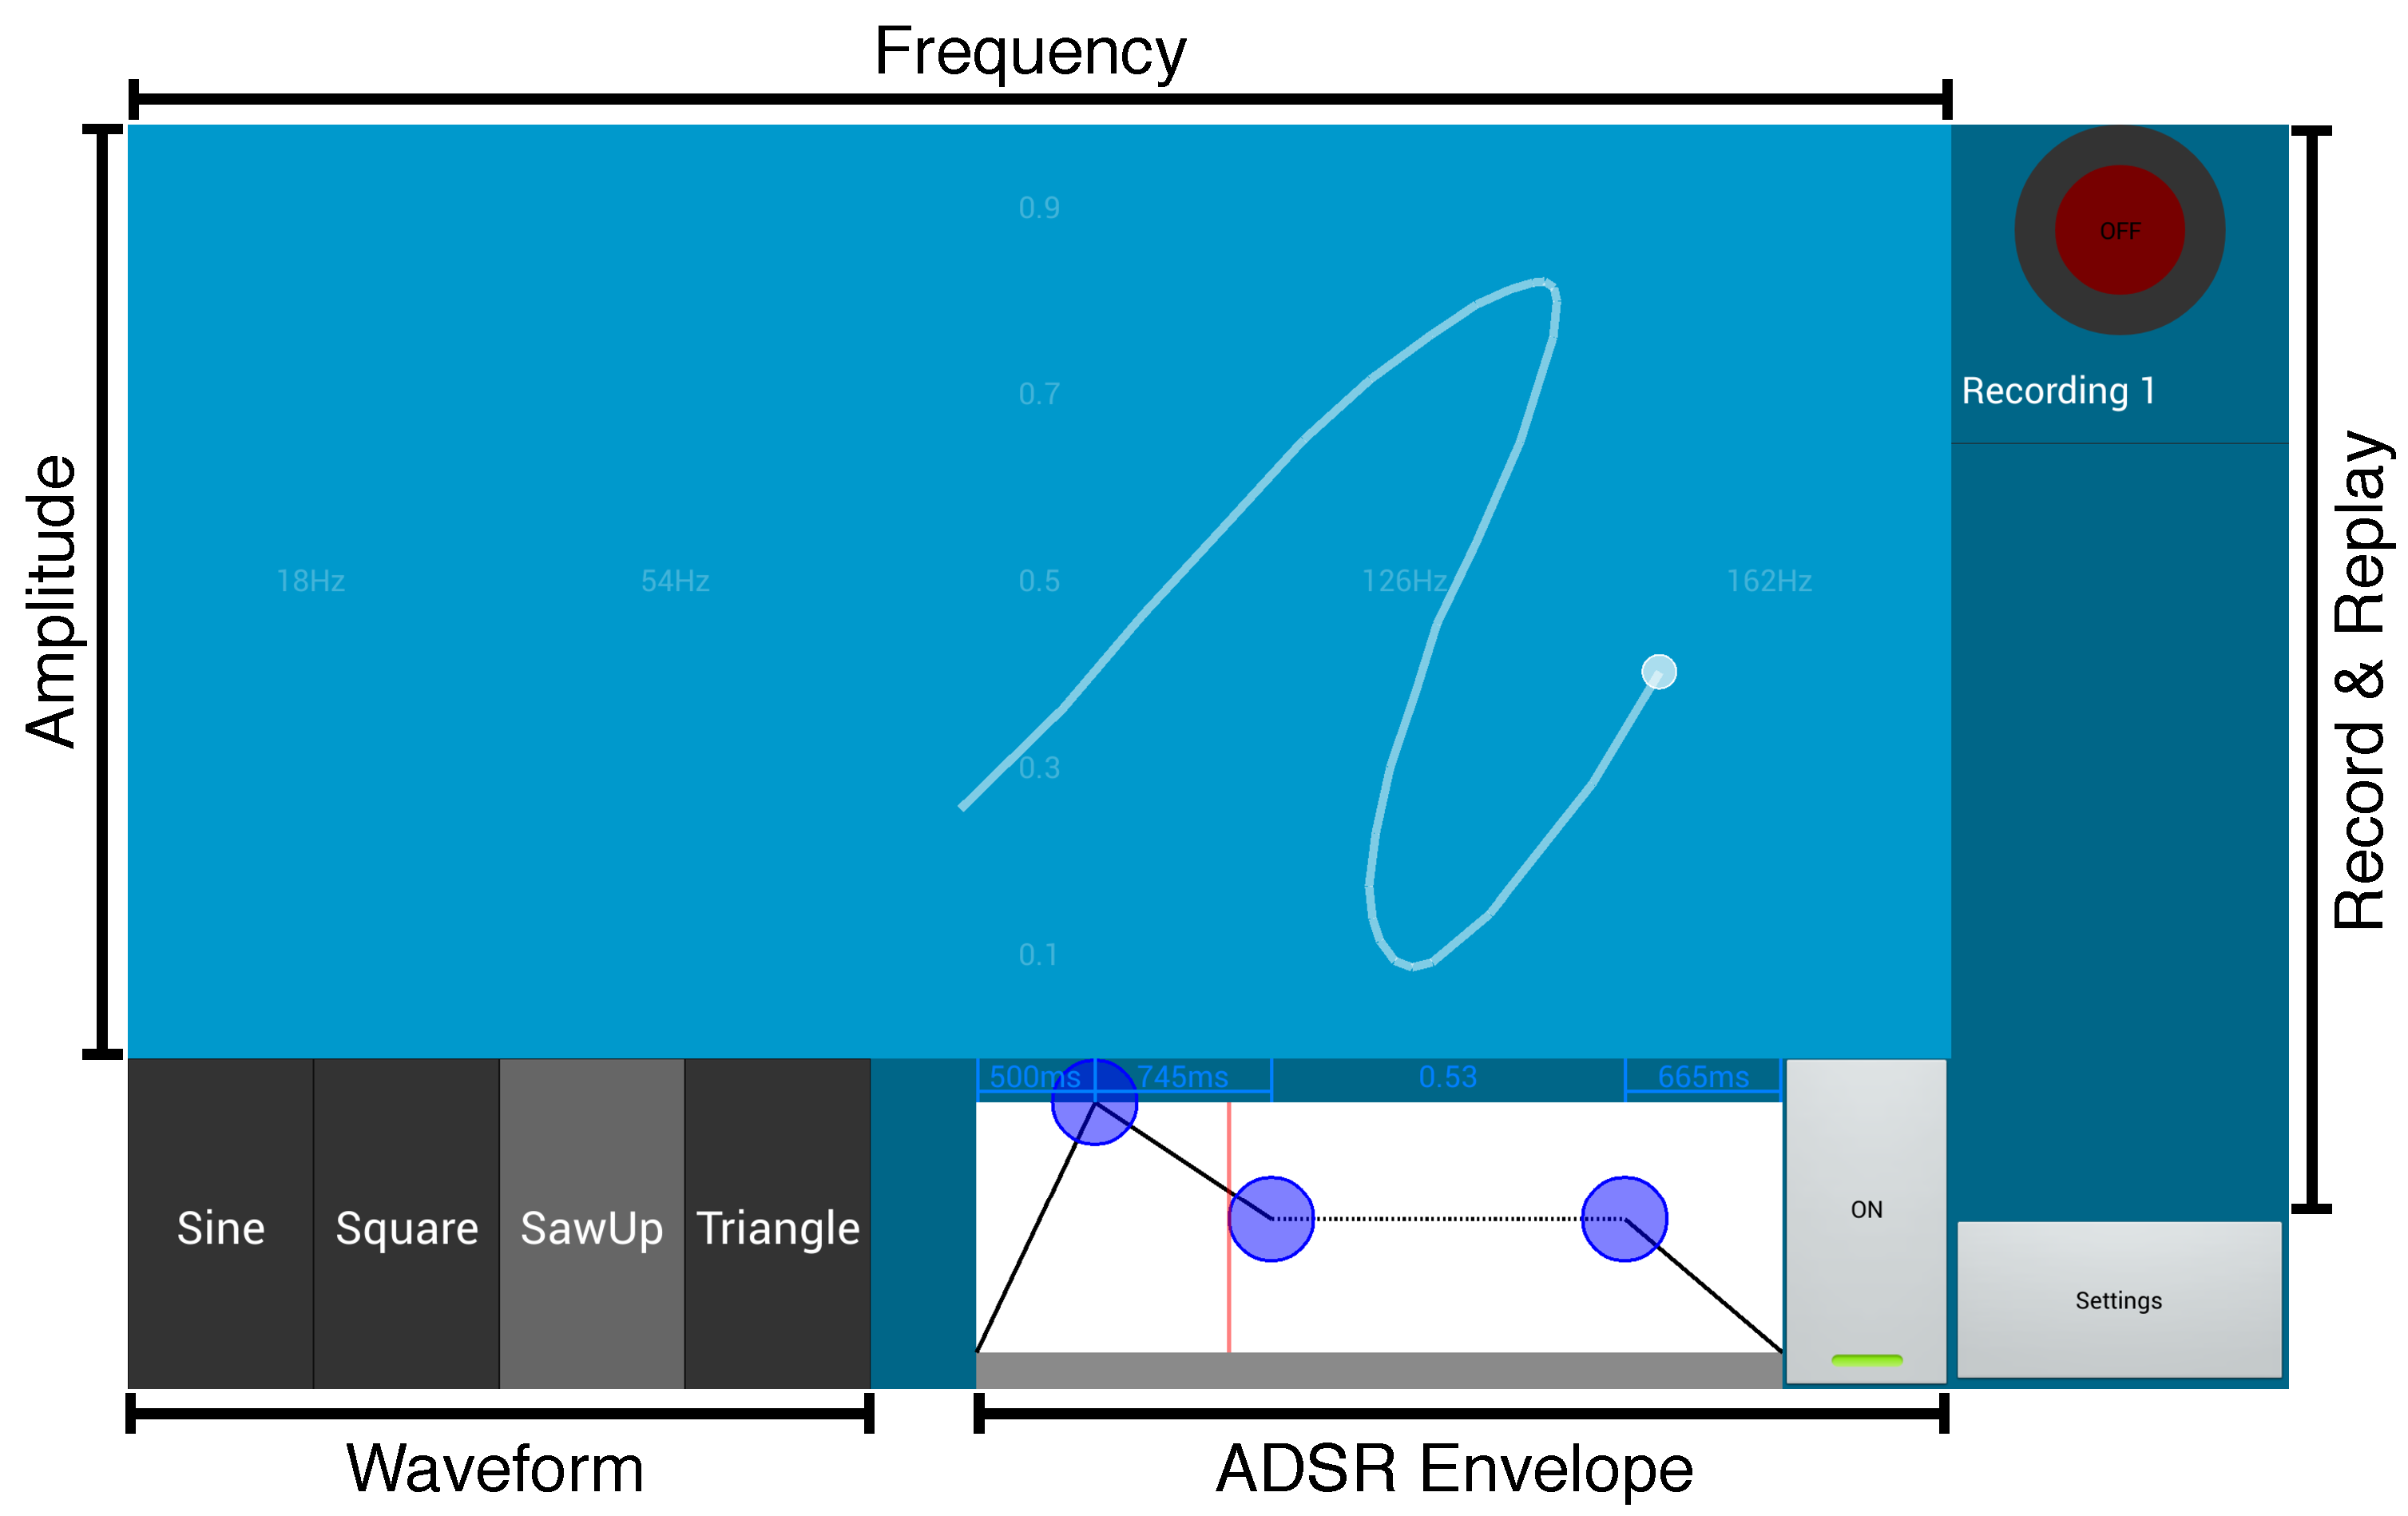
\includegraphics[width=0.43\textwidth]{mHIVE-screenshot-labeled-2013-08-13} 
	   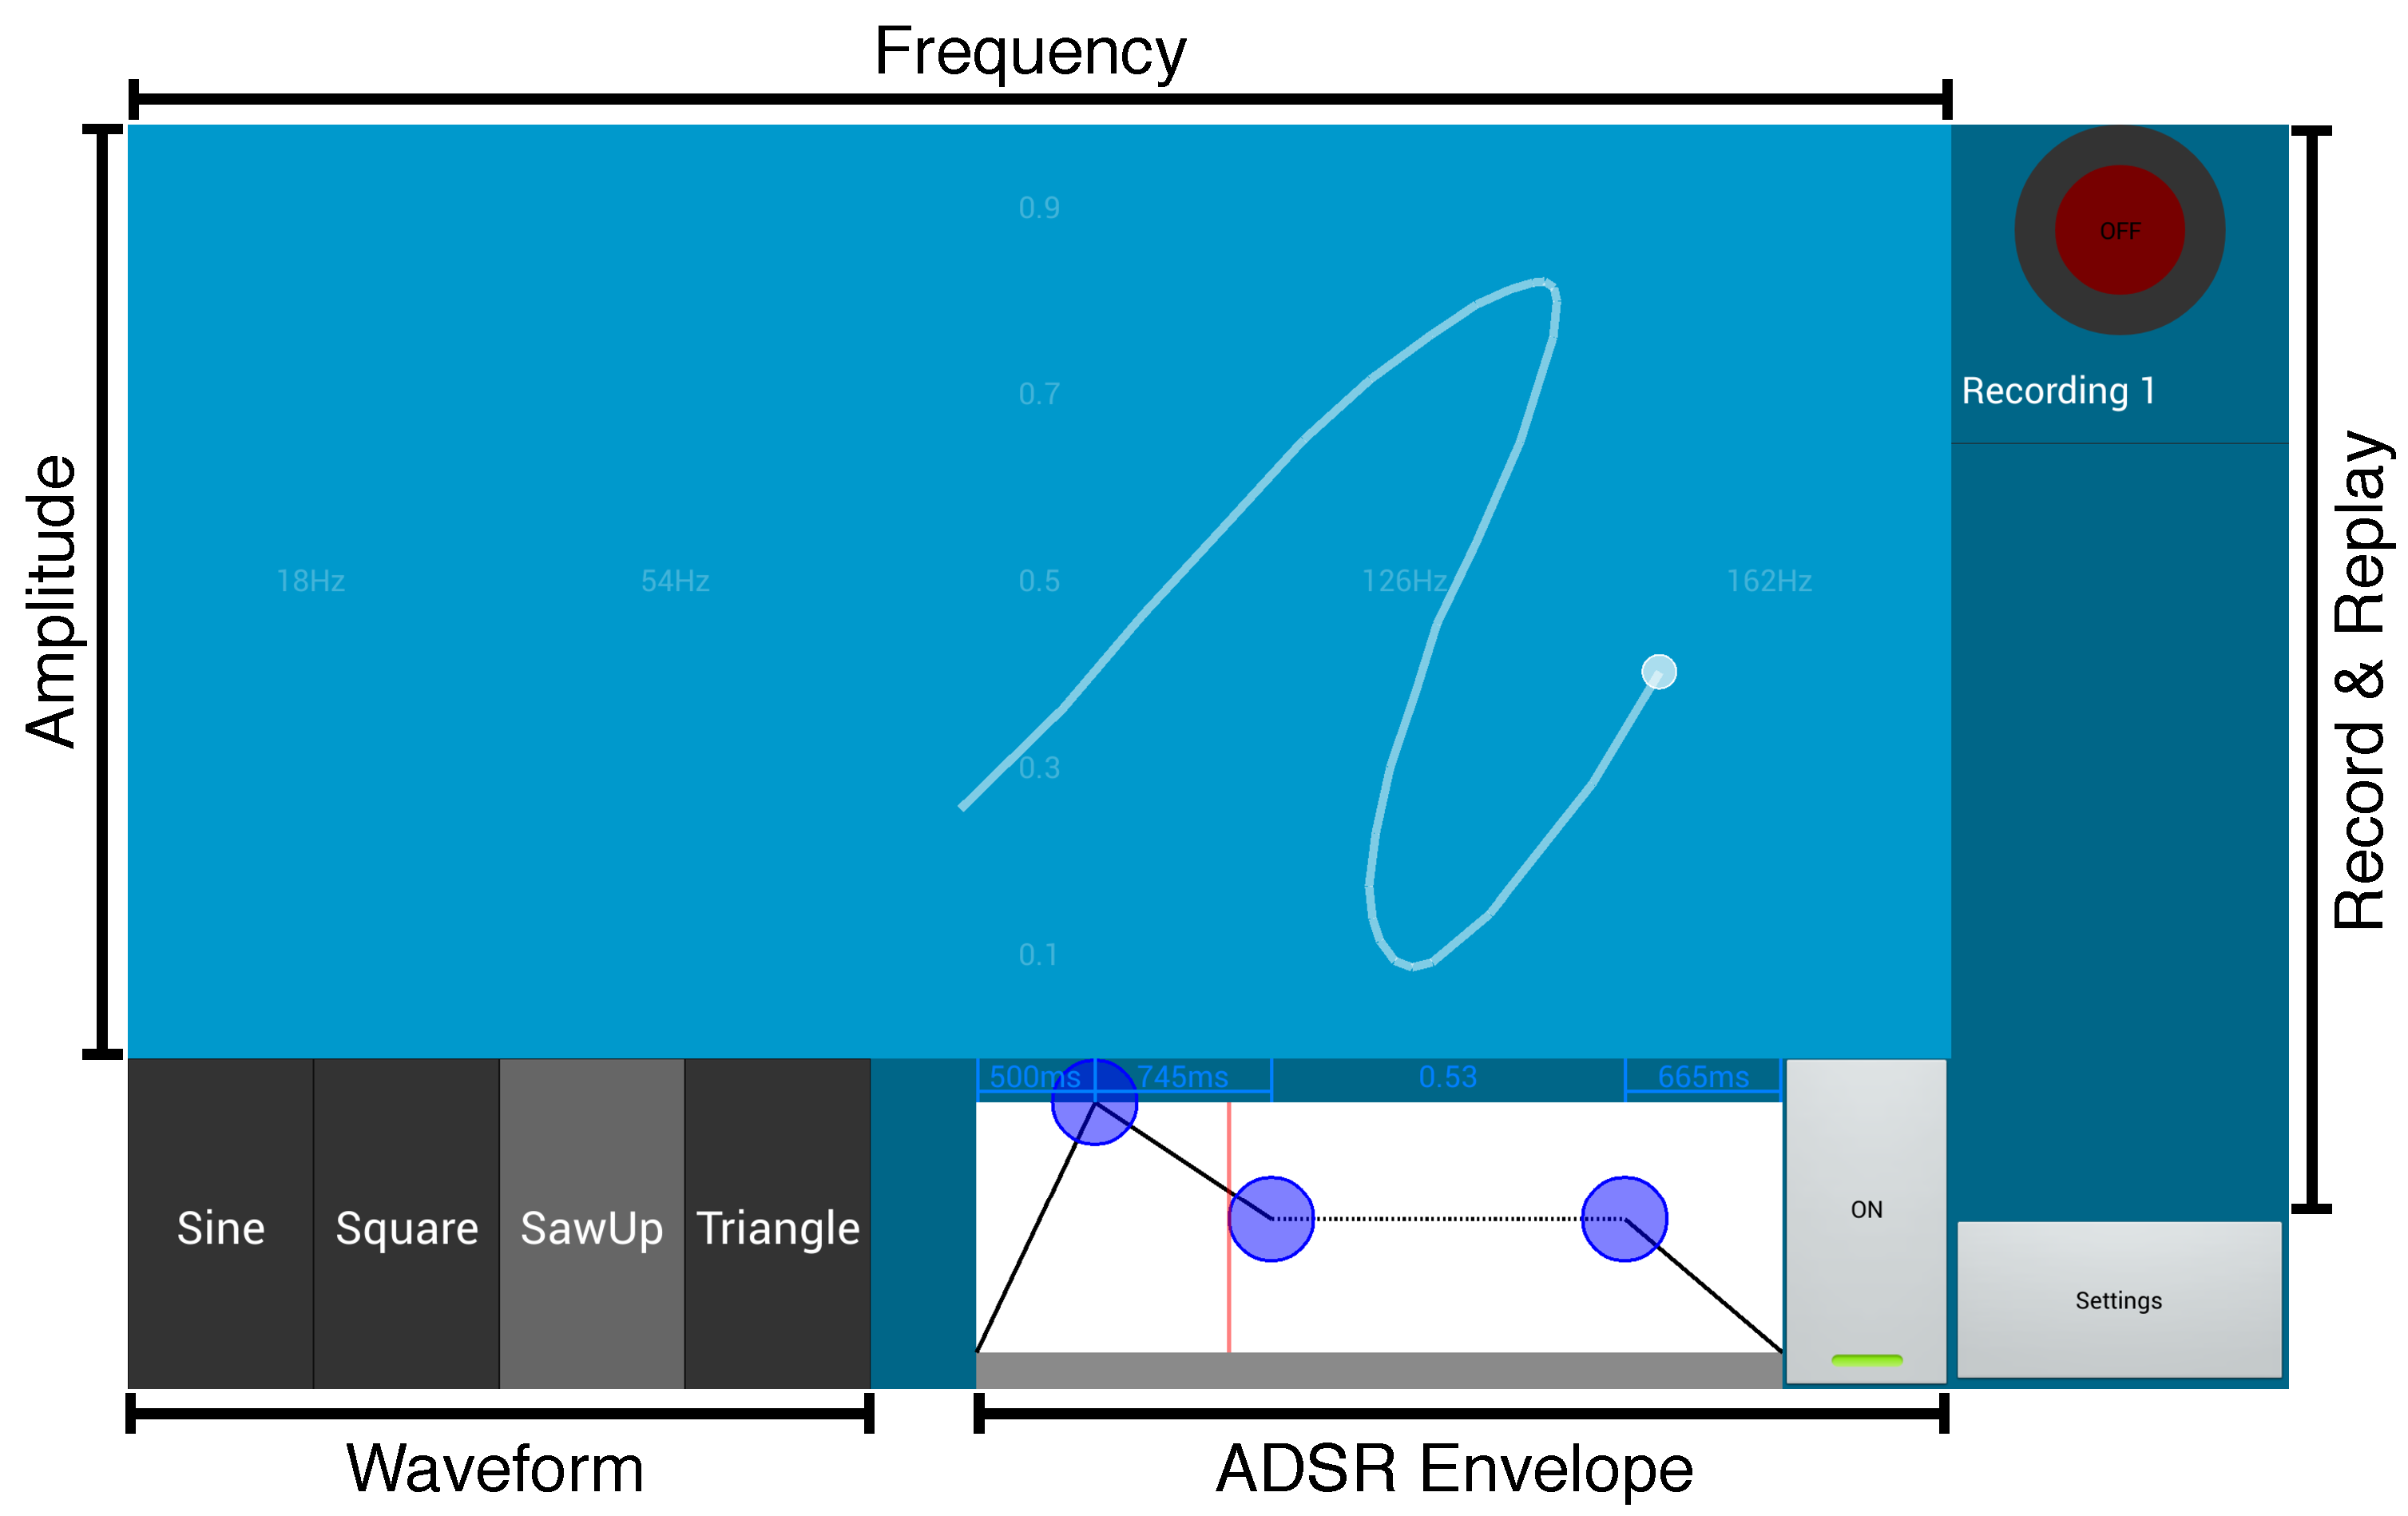
\includegraphics[width=0.7\textwidth]{mHIVE-screenshot-labeled-2013-08-13} 
	   \caption{mHIVE interface. Primary interaction is through the amplitude-frequency view, where visual feedback is provided through a circle (current finger position) and a trail (interaction history).}
	   \label{fig:mHIVE}
    \end{figure}


mHIVE offers real-time control of frequency, amplitude, waveform, envelope, duration, and rhythm, identified as the most important parameters for VT sensations \cite{Gunther2002,Brown2006a,Brown2006,Brewster2004, Rovan2000}.
mHIVE is implemented in Java using the Android SDK \cite{AndroidOpenSourceProject2012}, and the FMOD sound synthesis library \cite{fmod2013} to produce sounds, sent to two or more Haptuators through an audio jack.
%Thus, mHIVE is effectively a sound synthesizer designed for tactile sensations.
We deployed mHIVE on an Android Nexus 10 tablet running Android 4.2.1.



%mHIVE allows for control of frequency (5-180Hz, determined through piloting) and amplitude (0 (min) to 1 (full)) by drawing on a main input canvas.
%The ADSR filter can be toggled on or off by an adjacent button.
%As well, mHIVE allows for the user to record their input for later play back.
%Recording captures all input events, including waveform selection, ADSR manipulation, frequency/amplitude input, and even recording playback.

%%%%%%%%%%%%%%%%%%
%
% SECTION: Study Methodology
% 
%%%%%%%%%%%%%%%%%%
%\clearpage
\section{Study}

% With mHIVE built, 
We conducted a preliminary qualitative study to investigate two questions.
%\km{Q1/Q2?slc} % consider numbering them for more structered reference later. gives a bit of formalism.
First, is mHIVE an effective tool for the expression, exploration, and communication of affective phenomena?
Second, what language, mental models, and metaphors do people use to describe VT sensations, and how do they relate to mHIVE's low-level control parameters?

\begin{figure}[tb]
	\centering
%	   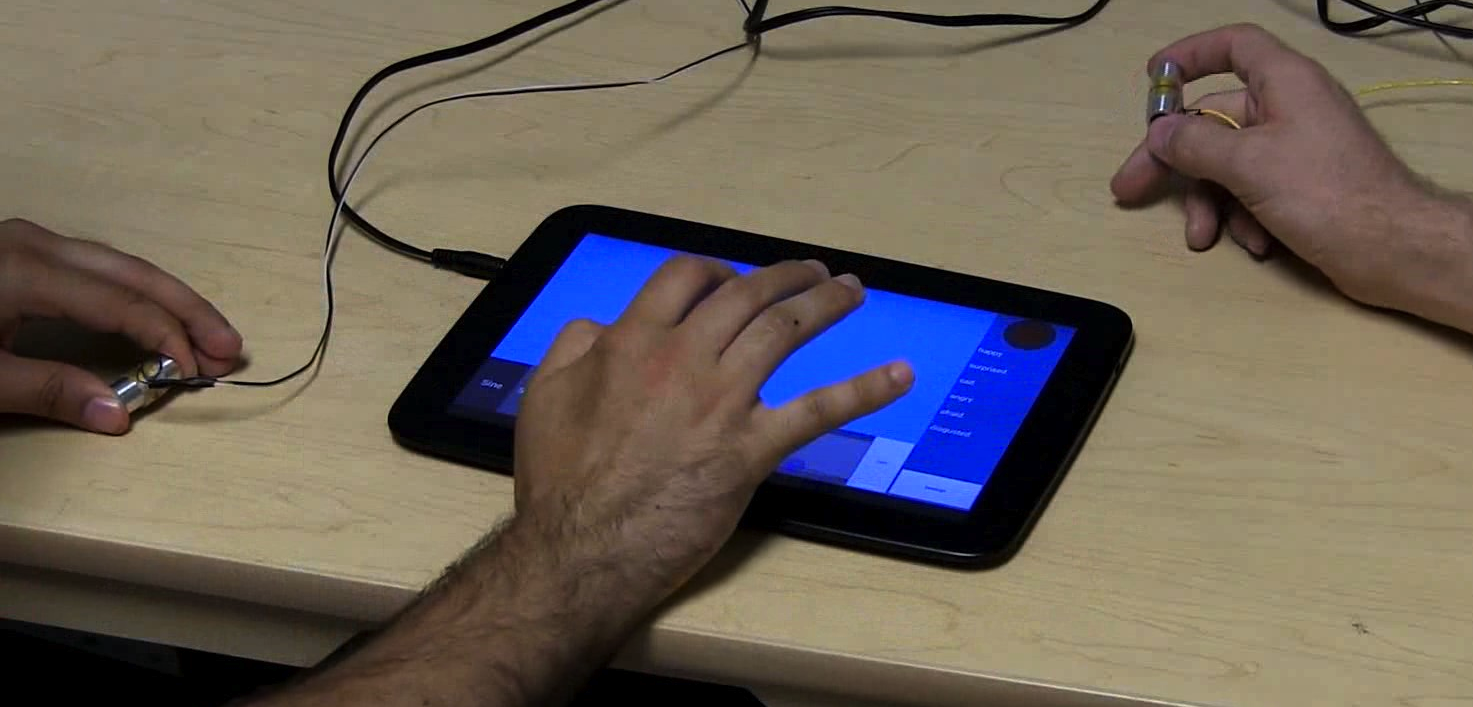
\includegraphics[width=0.32\textwidth]{mHIVE-study-setup-cropped2} 
	   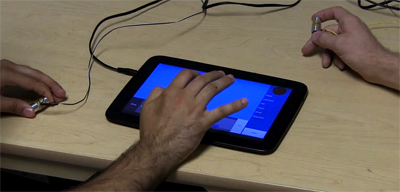
\includegraphics[width= 0.42\textwidth]{mHIVE-study-setup-cropped2small} 
	   \caption{
	   Study setup. Both the participant (left) and the interviewer (right) feel the same sensation as the participant controls mHIVE.
%	   The participant (left) controls mHIVE while feeling the sensation; the interviewer (right) feels the same sensation.
}
	   \label{fig:StudySetup}
\end{figure}

% \noindent
We collected and analyzed our data using the methodology of phenomenology, 
% a standard method
an established variant of qualitative inquiry used in psychology to investigate topics ranging from visual illusions to tactile experience \cite{Richer1978, Obrist2013, Creswell2013}, but always as a means to explore subjective experience.
%In particular, we use the Stevick-Colaizzi-Keen method as described by Moustakas \cite{Moustakas1994}.

Four participants were recruited through email lists and word-of-mouth (P1-4, three male, ages 26-35 with self-reported occupations including graduate students or post-docs in information visualization, HCI, and human-robot interaction).
All had experience working with haptic technology.
%, and (because of this requirement) all knew the main researcher in a professional capacity, although only P2 had seen earlier prototypes of the haptic instrument.
The small sample size, typical for phenomenological studies \cite{Creswell2013}, was appropriate for the rich data we wanted.
Data collection ended when we achieved saturation of new results, and had a clear direction for future iterations.


\section{Results}



%Phenomenology explores subjective experience, appropriate for an investigation into the more intangible qualities of pleasantness and affect.
%At this point, the rich, inductive data of qualitative analysis is more valuable than a controlled experiment with statistical analysis.
%We chose this over more familiar statistical methods because we have no established interfaces or task examples for haptic design.
%As such, any measures of error rate or time are meaningless.

%In particular, we use the Stevick-Colaizzi-Keen method as described by Moustakas \cite{Moustakas1994}.
%In-depth interviews are conducted with a small number of participants.
%The interviewer, Researcher 1 (R1), also documents his experience, as if he was interviewing himself.
%Then, R1 transcribes each interview, including his own.
%Transcripts are divided into non-overlapping, non-redundant statements about the phenomena known as Meaning Units (MUs).
%This considers every statement that the participants make, and does not discount any due to bias or selective searching.
%%
%Then, MUs are clustered into emergent themes. %through affinity diagrams.}%, writing and re-writing of thematic descriptions, and reflection guided by phenomenological philosophy.}
%% KM: can you expand (1 sentence) on this clustering and what follows? to address the concern of being biased or selective in comments. Need more transparency on what this part of process is.}
%%
%%Throughout the process, the philosophical principles of phenomenology are kept in mind; see \cite{Moustakas1994} for more detail.
%We interpret our themes in the Discussion.

%\subsection{Procedure}
%Our 1-hour open-ended interviews
%%with four participants, all with haptic experience.
%used the following protocol:
%\begin{enumerate}
%	\item Ask the participant for their background: occupation, experience with touchscreens, haptics, music, and video games.
%	\item Demonstrate mHIVE to the user, and invite them to explore while thinking aloud to describe the sensations they feel.
%	\item Probe the design space by asking participants to explore different control parameters, and to explore their metaphors (\emph{e.g.}, if the participant describes a sensation as ``smooth", R1 would ask them to try to produce a ``rough" sensation).
%	\item Ask the participants to produce sensations for the six basic cross-cultural emotions documented by Ekman \cite{Ekman1992}, and rank how well they think their sensation represents the emotion on a 4-point semantic differential scale (Very Poorly, Somewhat Poorly, Somewhat Well, Well). This was done both as an elicitation device to gather a wider range of interactions with mHIVE, and to directly investigate a design task.
%	\item Set the Haptuators down, and ask the participants to describe their experience of working with mHIVE in as complete detail as possible to evaluate the device itself.
%\end{enumerate}
%
%\noindent
%R1 conducted the interviews and analysis, which required specialized knowledge of mHIVE.
%%, and inductive nature of analysis did not allow for other researchers to cluster separately.
%% Because clustering was conducted and not coding, 
%%\kmEdit{Because we conducted clustering rather than coding,??}
%Scores of inter-rater reliability common with other qualitative analyses (\emph{e.g.}, grounded theory \cite{Corbin2008}) are inappropriate and unavailable, as we did not conduct deductive, low-level coding.
%To improve reliability,  R1's documented experience was analyzed first, and then consulted during analysis to remove bias (\emph{e.g.}, to not use terms only used by the experimenter).
%%documented and analyzed his own experience with the device, which was considered when conducting analysis.
%%we present here separately from other results to clearly demarcate the researcher's biases and preconceptions.
%%Even so, results are grounded in empirical data, shown by quotations representing the clusters.
%%Participants will also be contacted after analysis to provide feedback on our initial conclusions \textbf{TODO}.
%
%%%%%%%%%%%%%%%%%%
%
% SECTION: Results
% 
%%%%%%%%%%%%%%%%%%
%\section{Results}
%
%We sought participants with experience designing haptics as a proxy for expert designers for our initial study.
%Four participants were recruited through email lists and word-of-mouth (P1-4, three male), and were all in the age range of 26-35 with self-reported occupations including graduate students or post-docs in information visualization, HCI, and human-robot interaction).
%All had experience working with haptic technology, and (because of this requirement) all knew the main researcher in a professional capacity, although only P2 had seen earlier prototypes of the haptic instrument.
%The small sample size, typical for phenomenological studies \cite{Creswell2013}, was appropriate for the rich data we wanted.
%Data collection ended when we achieved saturation of new results, and had a clear direction for our next iteration.

%determined by saturation of new data: when we stopped encountering new data, we stopped recruiting participants.

%Analysis revealed several themes among the participants, particularly about the device's role in the design process, a tendency towards audio metaphors or concrete example-based metaphors, and a notion of enjoyable sensations vs. non-enjoyable sensations.
%As well, usability concerns are reported, suggesting implications for the design of future haptic instruments.

%
% Subsection: Reflections
%
%\subsection{Researcher Reflections and Experience}

%\emph{Note: This section is written by the researcher who led development of mHIVE and conducted the interviews and analysis.}

%%Researcher eval v1
%%As the principle developer of mHIVE, I have a unique outlook on the device.
%%I entered the study with planned improvements derived from piloting.
%%Deliberate exploration of the device revealed a number of takeaways which I will report here.
%%Some are may be similar to the experience reported by study participants, and some are specific to me.

%%Because I built the device, I understood the underlying mental model, and thus found mHIVE to be \q{very intuitive,} and \q{very helpful.}
%%I \q{enjoyed using it.}
%%I found visual trace and ADSR envelope to be \q{helpful.}
%%In particular, ADSR was very \q{important} to me, and was useful to \q{soften the edges} of the sensations.

%%However, I do not believe that mHIVE is perfect.
%%First, the addition of multitouch is \q{important.}
%%I found it was tricky to \q{juggle both hands}, feeling the output while simultaneously controlling the interface.
%%I have mixed feelings about the recording feature. Though I found it \q{helpful the one time} when developing the surprise sensation, I only used it once and feel that it \q{needs work.}
%%I had originally though that the recording feature needed a stop button, but \q{I didn't used it enough to notice} any lack of such a feature.

%%Finally, I found myself changing waveform and ADSR infrequently; it was \q{easy to leave something in place.}
%%Overall, I felt that mHIVE was \q{an exploratory tool} rather than a tool for \q{refinement.}
%%It would be best suited to exporting icons to \q{another application or another task.}

%%researcher eval v2
%Because I built the app, I understood the underlying system model. Because of this, I enjoyed using it, thought it was helpful, and found it intuitive and easy-to-use. I thought visual trail was very nice and helpful, because I could see where it was, and that ADSR was important, especially for a ringing sensation. I experienced unexpected sensations, calling them weird.

%Of course, because I was using an early prototype, there were still some interface-level refinements I thought were important to make. Some of these became less important as I interacted with the device. I thought that it needed a button to stop replay, but because I only used the record/replay feature once when exploring the device and didn't notice the lack of a stop button, I thought it was fine. Interacting with the device, multitouch emerged as an important feature to try. Overall, I though mHIVE was suited for exploration but not refinement, and thought it might be a good idea to record haptic icons and export them to another application.

%Low frequency sensations stood out to me as oscillating, pushes, thumps or hits (with the square wave), and felt like a watch or subwoofer. I described some low-level sensations with onomatopoeias, including djoo djoo djoo, wub wub wub, tick tick tick tick. ADSR allowed sensations that felt like soft bells, and that made me picture the sound of an ocean swelling. I made frequent analogies to technology: lasers, boat motors revving, and zippers, and could hear higher frequencies, comparing them to mosquitos buzzing or high pitched whines like an plane engine.

%I also used tactile metaphors, tingly, strained, taut, grainy, gritty, and rumbly. Triangle and sine waves became more forceful while square and sawtooth waves became stronger. Higher frequencies were smooth, like a constant ringing, and sometimes aggressive, viscious, on edge, or even painful (on one occasion).

%
% Subsection: Themes
%
%\subsection{Themes}
In this section, we outline the three major themes that emerged during analysis: % possibly: use this spot to help with the expansion on methodology, reinforcing that it was systematic not biased, clearly a concern of the reviewers.}
%
 mHIVE's success as a haptic instrument, mHIVE's limitations that reveal more detail about the haptic design process, and the use of language in the study.

%\theme{mHIVE Succeeds as a Haptic Instrument}

Our results suggest that mHIVE was well received and \textbf{succeeded as a haptic instrument}. %, and can be effective for exploration of a design space and communication in the haptic domain. % This section 
Participants reported that mHIVE was best served to explore the design space, generate a number of ideas, and \nq{2}{accidentally stumble upon something} as they explored the device.
mHIVE also
established an additional modality for dialogue.
The dual outputs created a shared context, demonstrated by deictic phrases: the additional context of the VT sensation was required to make sense of the statements like  ``that" and ``there".
%, reminiscent of the classic ``Put That There" multimodal interaction demo \cite{Bolt1980} indicate a shared reference point was established from the haptic instrument.

%theme 2
The second theme, \textbf{tweaking through visualization and modification}, established
key directions for future design.
Though mHIVE supported exploration and collaboration, we found 
it was inadequate as a standalone design tool.
Few created sensations were considered to be final,
%Many descriptions were hedged 
%and in the design task, few sensations captured the emotional content well.
%Part of mHIVE's inability to support tweaking was
partly due to cognitive limitations for both memory and attention.
Participants found it difficult to remember what they had tried before, 
and to pay attention to the output 
while simultaneously controlling it. 
%Participants suggested that although 
Participants suggested additional visualization and recording features, % helped somewhat
%to overcome these limitations, more was needed.
%All  requested greater emphasis on recording through
such as repetition or looping, both to aid memory and allow for focus on the sensation independent of device control. 
Allowing persistent, modifiable sensations % and alternative visualizations
could also help participants overcome these limitations.


The final theme was that VT sensations have \textbf{a difficult language}.
Our study was too small to analyze language patterns in detail, but exposes emerging trends.
Participants often started with a statement of like or dislike rather than a description, with
pleasant sensations often including
ramp-in and ramp-out (``echo" or ``ringing") of the ADSR envelope or lower-frequency sensations.
%Longer, higher frequency without ramp-in and ramp-out were less pleasant.
Changes of waveform were noticeable but difficult to describe. %, Participants all noticed differences between waveforms, but were often challenged in expressing them
%(P4 
%used the musical term ``timbre").
%Square waves in particular were distinct, with a greater range and stronger affinity to mechanical sensations.
%\strongitem{Aural/haptic metaphors drawn from previous experience}
Participants also frequently 
%For the most part, participants 
used concrete examples and direct analogies to describe sensations, often drawn from their previous experiences.
One stand-out strategy employed by all participants  
was  
onomatopoeias (e.g.,  \nq{1\&4}{beeooo}).
%, \nq{1}{vroom}, \sq{bsheeeooo}, \sq{boom}, \sq{neeeaa}, \nq{2}{mmmMMMmmm}, \sq{pa pa pa pa}, \sq{tum tum tum tum}, \nq{3}{tumba tumba tumba tumba}; \nq{4}{upward arpeggio, like, (singing with hand gestures) na na na naaa}.
Other common metaphors were sound-based %( %including hum, buzz, whistle, rumble (P1);
(e.g., \nq{1\&2}{bell})
%; squeaky, creak (P2); or
%thumpy (P3).
%Still other descriptors were directly haptic in nature:
or haptic
%rough, flat (P1);
%sharp, round, ticklish (P2);
(e.g., \nq{3}{cat pawing}).
%sharp, smooth, cat pawing (P3);
%impatient foot tapping (P4).




%%%%%%%%%%%%%%%%%%
%
% SECTION: Discussion
% 
%%%%%%%%%%%%%%%%%%
\section{Discussion}
Ultimately,
mHIVE was able to achieve the two main goals of a haptic instrument, facilitating both exploration and collaboration, which showed value in real-time exploration and a shared output context.
mHIVE also had limitations - participants could not edit sensations and found it difficult to keep track of multiple sensations.
This is understandable given the broader context of the musical instrument analogy we used for inspiration.
Musical instruments are not used to write songs on their own, but % need to be 
combined with notation or recording media.
There may be no silver bullet with haptic design tools, with haptic instruments solving a particular set of processes (quick, easy ideation and communication for experts) but not others (final touches, distribution).
Ultimately, haptic instruments may be most useful as one element
% might be useful as one type of tool  % 
in a suite, or component of a more general tool.
%A designer could keep a haptic instrument to quickly sketch ideas while working with a more heavyweight tool that allows for manipulation of a haptic sensation.
%This could be in an ``exploration mode", or perhaps a portable tool to sketch ideas when not near a haptic editing suite.

We follow-up on these leads in our subsequent design studies.
In \autoref{ch:hapticanimation}, we use a persistent model of a VT sensation for an editor, and confirm the value of real-time feedback while expanding the design palette to include spatial haptics.
In \autoref{ch:hapticexamples}, we attempt to mitigate the difficulty of describing haptics and draw upon examples by using a VT design gallery.




%Participants were clearly able to explore the different low-level parameters, and encountered serendipitous or unexpected sensations through improvisation.
%mHIVE created a shared experience that facilitated communication between R1 and the participants.
%We can thus conclude that haptic instruments are a promising new tool in a haptic designer's arsenal, with a first, successful implementation in mHIVE.

%However, the second theme shows that serendipity and communication are only part of the equation.
%mHIVE does not serve as a general editor of haptic sensations.
%In particular, participants found their attention split when controlling the device and feeling the sensation; perhaps the real-time control should allow for a rapid, but not instantaneous, switch in focus between control and perception.
%More generally, participants were unable to tweak sensations because there was insufficient support for comparing ideas or evolving an existing idea.
%
%
%A similar combination of a haptic instrument and recording might be described more succinctly as %with
% a \emph{haptic sketchpad}.
%Sketching is critical in design because it allows for the evolution of an idea through multiple sketches, as well as criticisms, comparisons, and modifications \cite{Cross2011}.
%%By adopting a more visual, modifiable tool, we can support tweaking.
%Emphasizing a history feature that supports multiple versions of sketches, the user could develop an idea as if with a multiple pages in a sketchbook.
%Haptic sketching in hardware has already been shown to be %very 
%effective \cite{Moussette2011}.  %; we plan to explore more visual metaphors with future iterations.
%As well, a visual metaphor resonates with the desire for more effective visualization.
%%, so a software perspective might be promising
%%A haptic sketchpad would make heavier use of visual working memory to offset the noted perceptual-cognitive challenges with .
%%Of course, effective visualizations are challenging, and are left to future work.

%Ultimately, haptic instruments may be most useful as one element
%% might be useful as one type of tool  % 
%in a suite, or component of a more general tool.
%% As part of a suite of tools, mHIVE or other 
%A haptic instrument could complement % work together with 
%a graphical editing tool that does support tweaking, such as the vibrotactile score \cite{Lee2012,Lee2009} or the hapticon editor \cite{Enriquez2003}.
%%This path mirrors musical development directly, and so more inspiration might be from digital audio tools.
%As part of a more comprehensive tool, mHIVE could be improved to reduce cognitive barriers to memory and attention.
%Alternatively, we could add functionality to mHIVE to support looping, visualization, and direct manipulation of the sensations within the tool.
%Many of these results fed into the next case study, Tactile Animation, which expanded to include space and time as controlled dimensions.


\endinput
